
\section{katz-eig}\label{sec:graphs:katz-eig}

\Warning[TODO]{ title? Where? What? How? :) }

\textit{Also final runtime to find beta/K for different datasets?}

\textit{alpha}, \textit{alpha2} and \textit{eswc2015music} were too slow to run on my computer.
\Warning[TODO]{ Describe system I test things on }


\subsection{Model selection}

These are plots for possible models with rank $K$ low-rank approximation for \textit{katz-eig}.  All plots use $\beta = \frac{1}{|h_{train}|}$ and evaluated using a top-10 top list.

\FloatBarrier

\begin{figure}[h!]
  \centering
    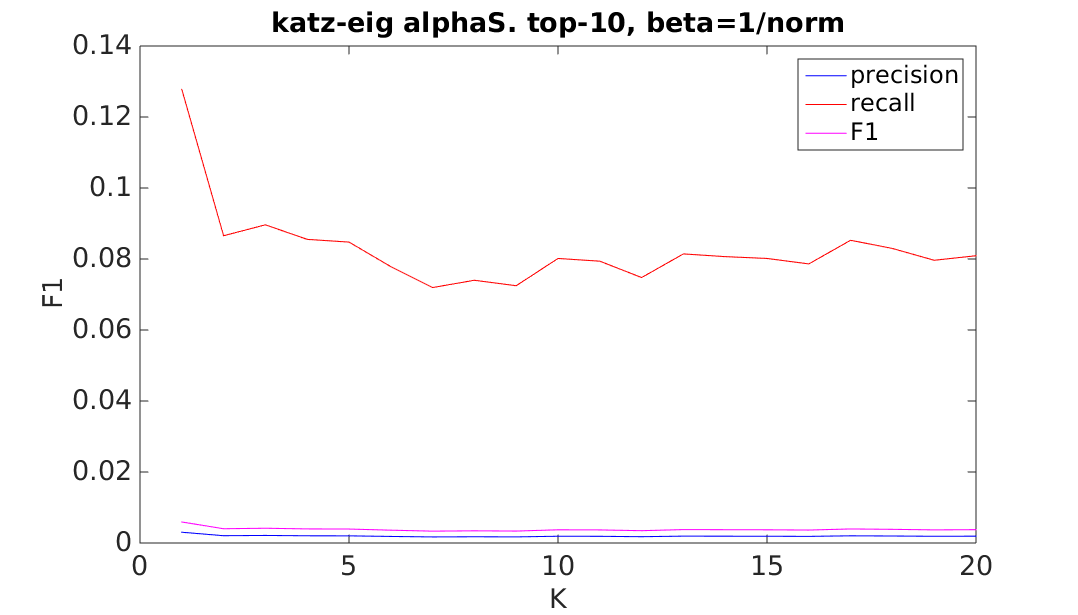
\includegraphics[width=0.9\textwidth]{fig/katzeig_k/alphaS_katzeig_K.png}
    \vspace{-20pt}
    \caption{\textit{alphaS}}
    \vspace{-10pt}
\end{figure}

\begin{figure}[h!]
  \centering
    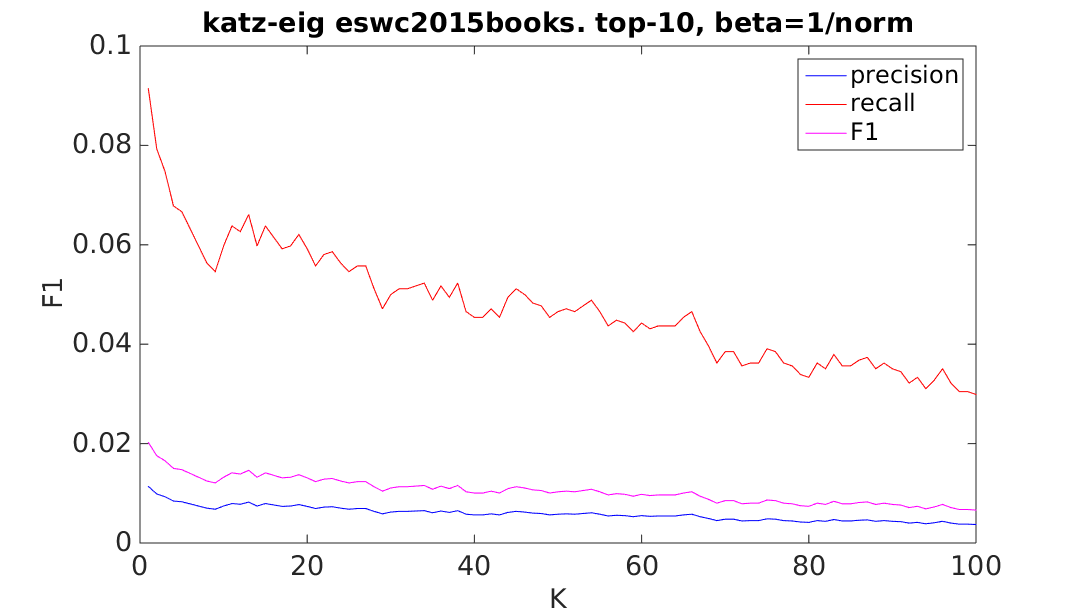
\includegraphics[width=0.9\textwidth]{fig/katzeig_k/eswc2015books_katzeig_K.png}
    \vspace{-20pt}
    \caption{\textit{eswc2015books}}
    \vspace{-10pt}
\end{figure}

\begin{figure}[h!]
  \centering
    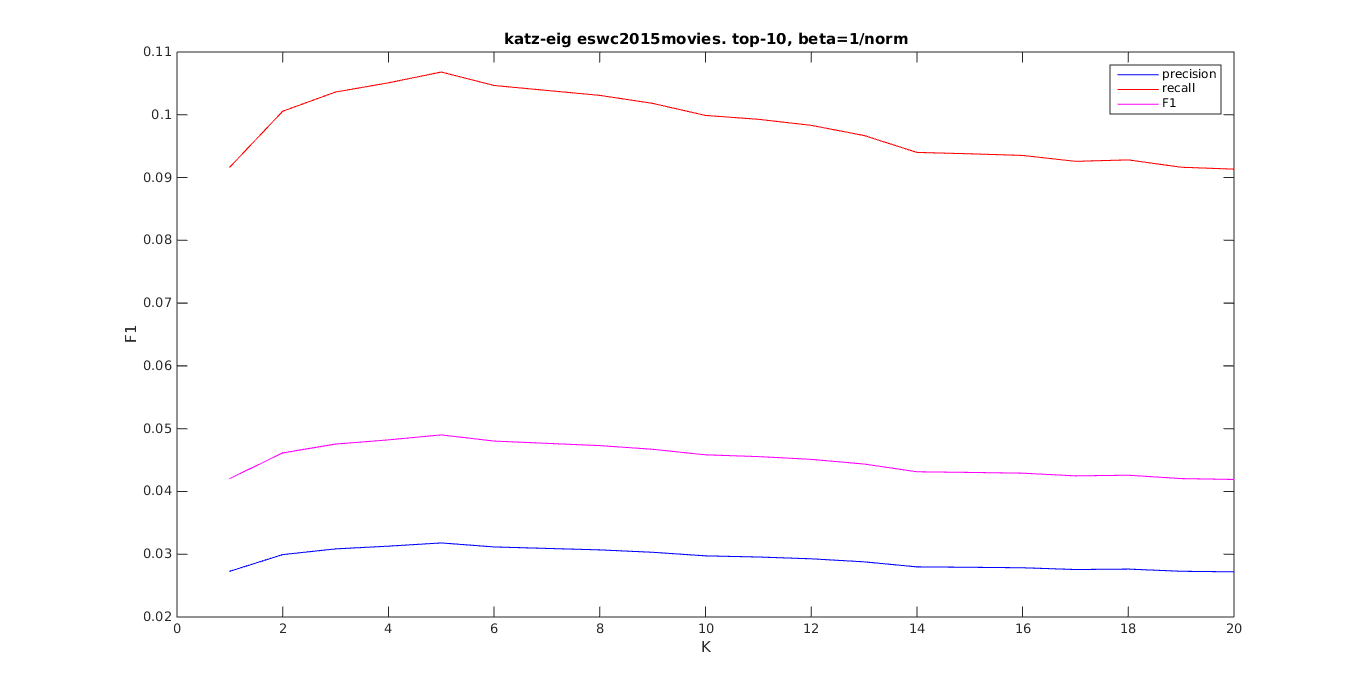
\includegraphics[width=0.9\textwidth]{fig/katzeig_k/eswc2015movies_katzeig_K.png}
    \vspace{-20pt}
    \caption{\textit{eswc2015movies}}
    \vspace{-10pt}
\end{figure}

\begin{figure}[h!]
  \centering
    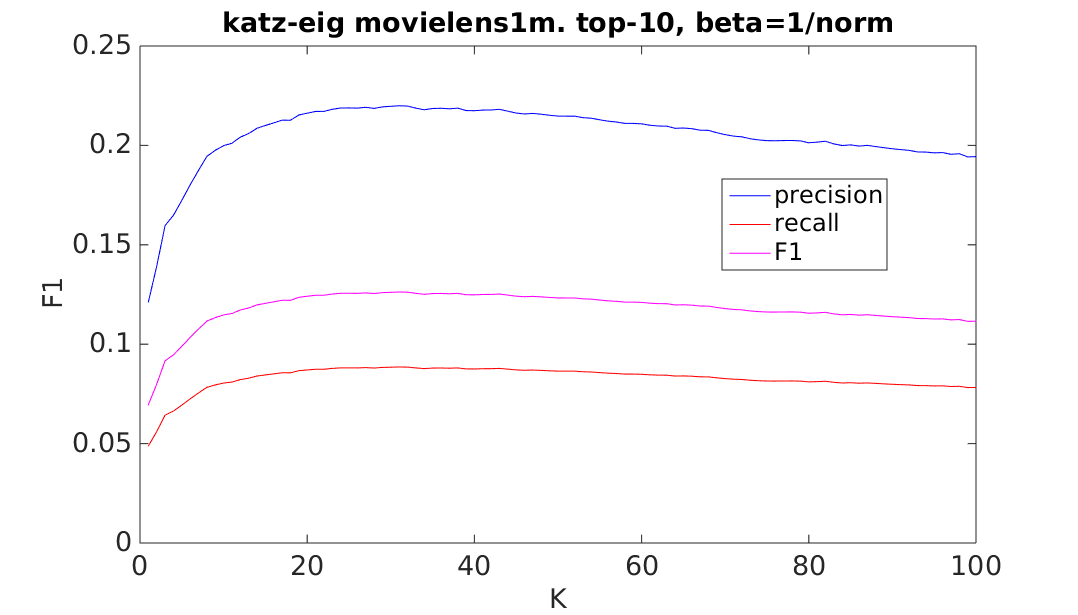
\includegraphics[width=0.9\textwidth]{fig/katzeig_k/movielens_katzeig_K.png}
    \vspace{-20pt}
    \caption{\textit{movielens1m}}
    \vspace{-10pt}
\end{figure}

\begin{figure}[h!]
  \centering
    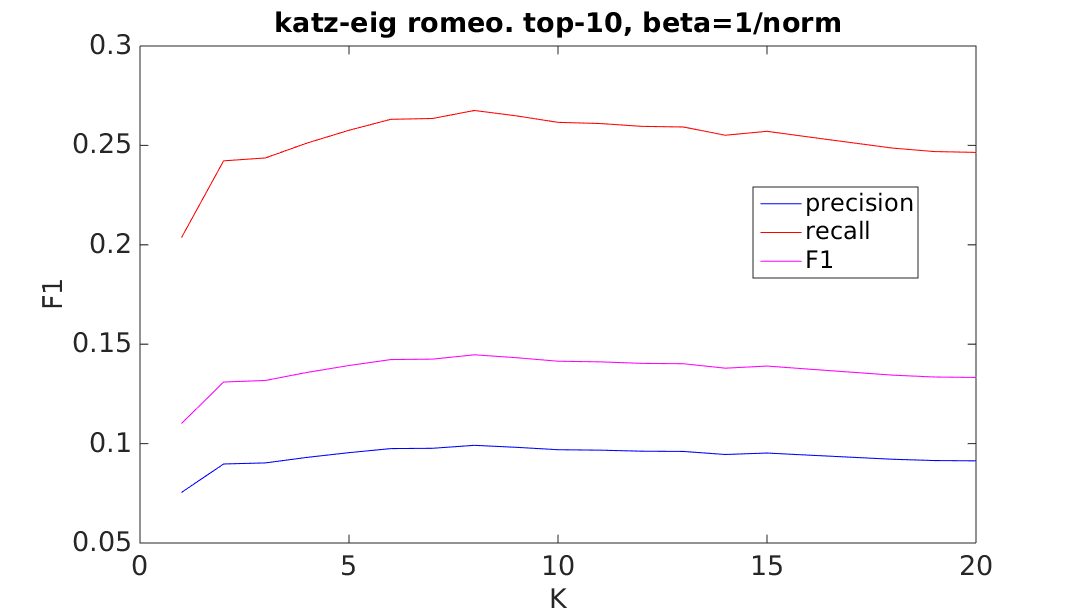
\includegraphics[width=0.9\textwidth]{fig/katzeig_k/romeo_katzeig_K.png}
    \vspace{-20pt}
    \caption{\textit{romeo}}
    \vspace{-10pt}
\end{figure}

\FloatBarrier


\subsection{katz-eig $\beta$}

These are plots for possible values of $\beta$ for \textit{katz-eig}. The values are plotted for the best $K$ for each dataset evaluated using $\beta_{max} = \frac{1}{|h_{train}|}$. Again evaluated for a top-10 list.

The range examined is $0 < \beta \leq \frac{1}{|h_{train}|}$.

\FloatBarrier

\begin{figure}[h!]
  \centering
    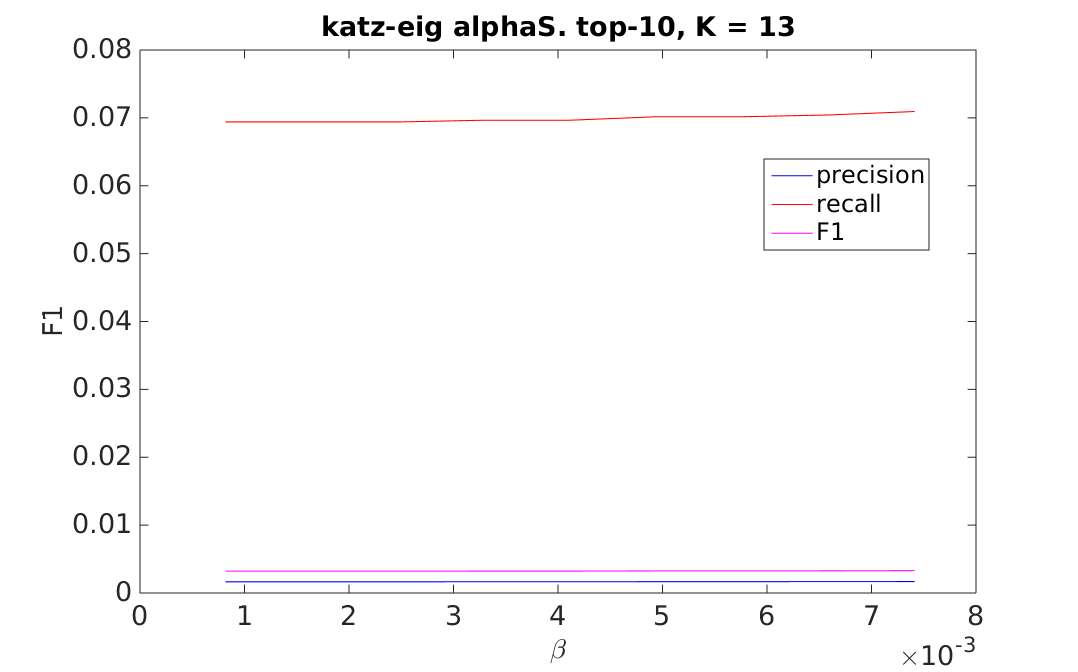
\includegraphics[width=0.9\textwidth]{fig/katzeig_beta/alphaS_katzeig_beta.png}
    \vspace{-20pt}
    \caption{\textit{alphaS}.
        $\beta_{max}$ is the best value with a $1.9\%$ diff between the minimum and the maximum \textit{F1} value.}
    \vspace{-10pt}
\end{figure}

\begin{figure}[h!]
  \centering
    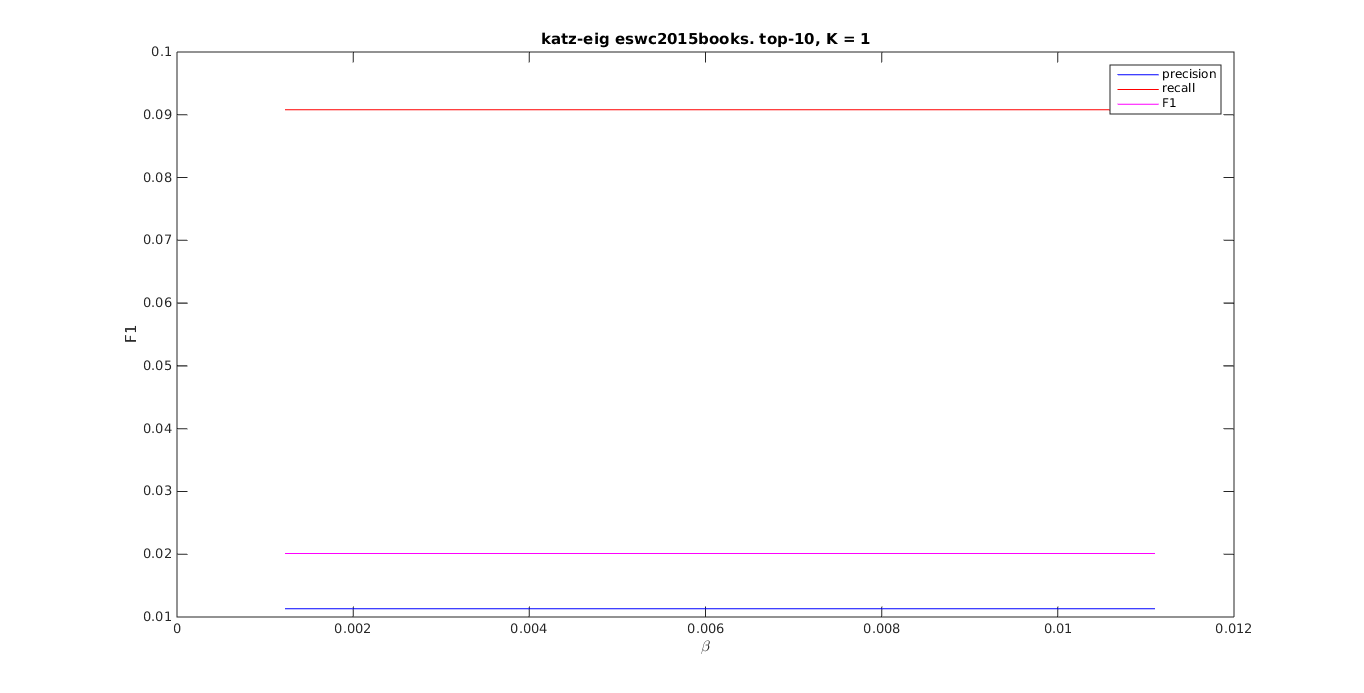
\includegraphics[width=0.9\textwidth]{fig/katzeig_beta/eswc2015books_katzeig_beta.png}
    \vspace{-20pt}
    \caption{\textit{eswc2015books}. All $\beta$ evaluate to the same value.}
\end{figure}

\begin{figure}[h!]
  \centering
    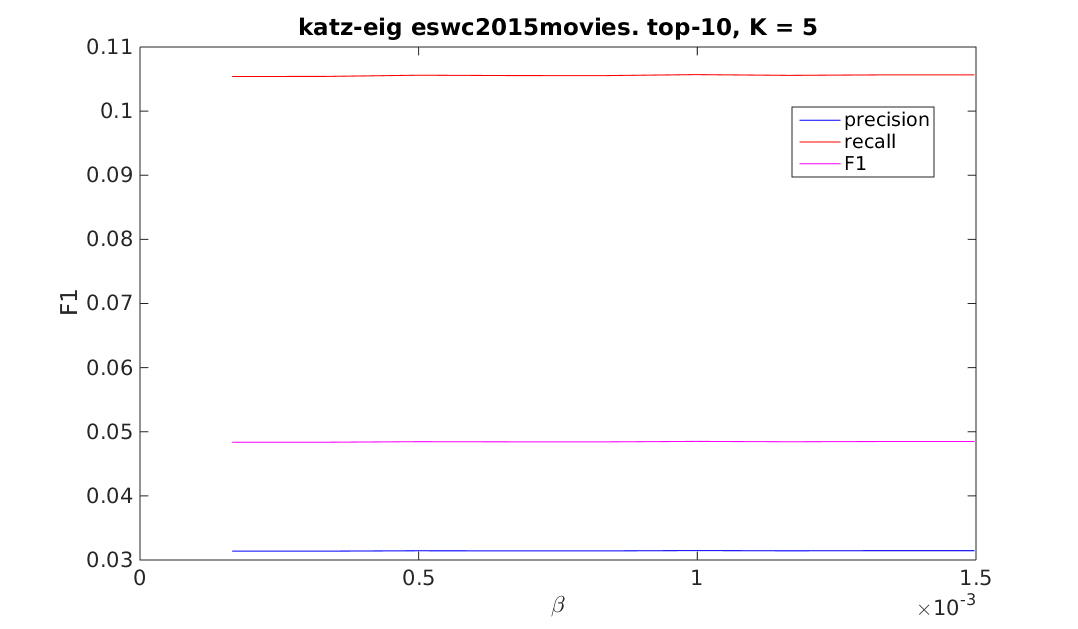
\includegraphics[width=0.9\textwidth]{fig/katzeig_beta/eswc2015movies_katzeig_beta.png}
    \vspace{-20pt}
    \caption{\textit{eswc2015movies}.
        $\beta_{max}$ is not the best value with a $0.3\%$ diff between the minimum and the maximum \textit{F1} value.}
    \vspace{-10pt}
\end{figure}

\begin{figure}[h!]
  \centering
    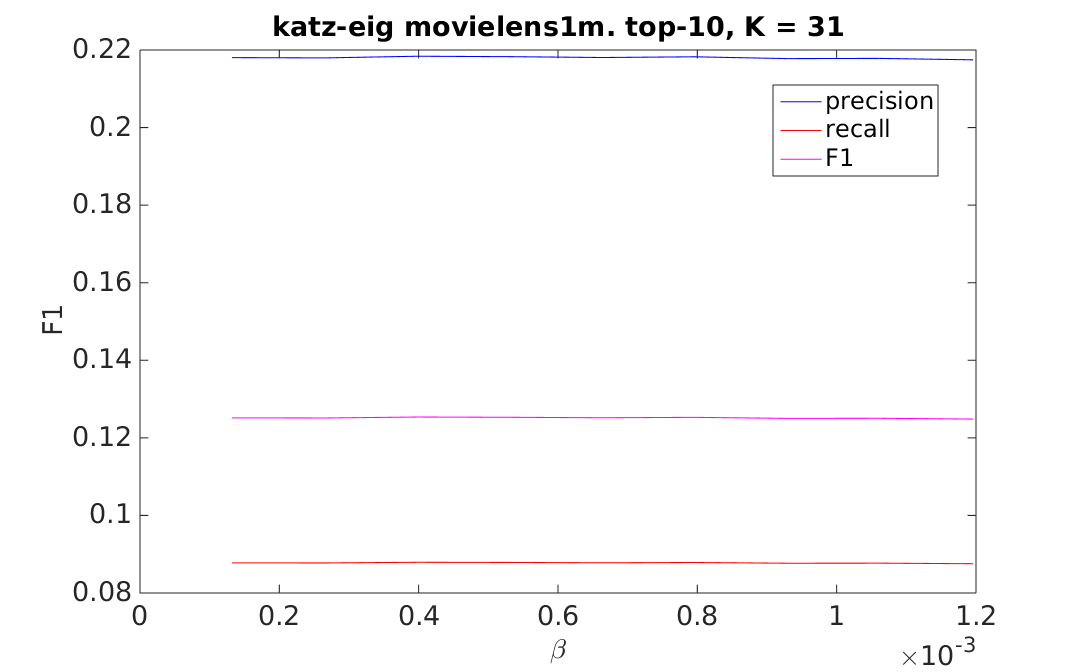
\includegraphics[width=0.9\textwidth]{fig/katzeig_beta/movielens_katzeig_beta.png}
    \vspace{-20pt}
    \caption{\textit{movielens1m}.
        $\beta_{max}$ is not the best value with a $0.41\%$ diff between the minimum and the maximum \textit{F1} value.}
    \vspace{-10pt}
\end{figure}

\begin{figure}[h!]
  \centering
    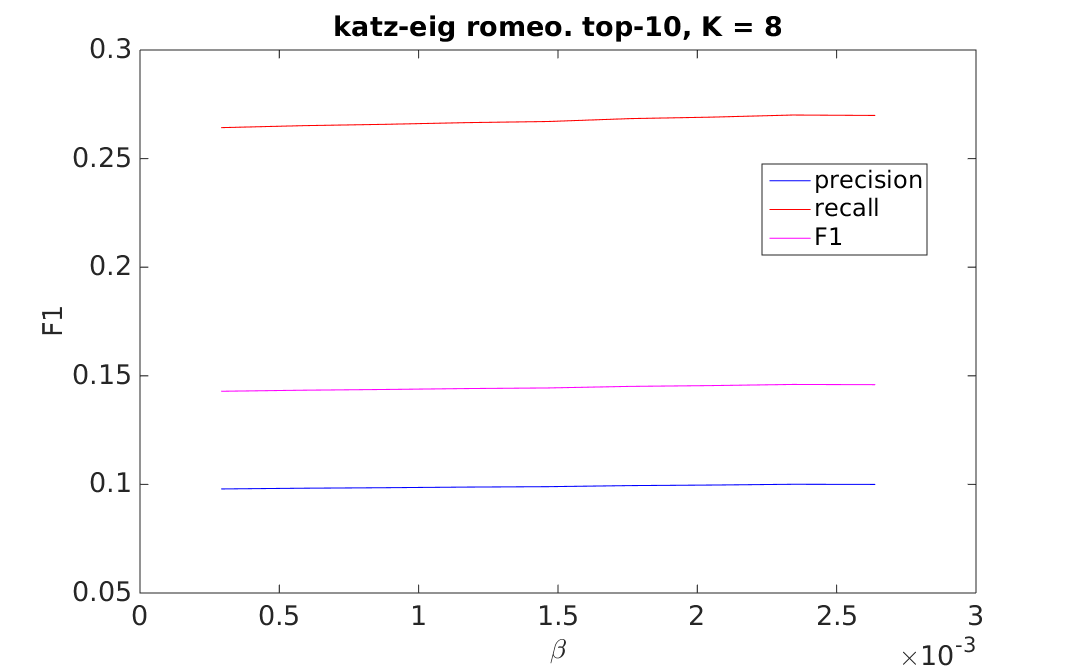
\includegraphics[width=0.9\textwidth]{fig/katzeig_beta/romeo_katzeig_beta.png}
    \vspace{-20pt}
    \caption{\textit{romeo}.
        $\beta_{max}$ is not the best value with a $2.09\%$ diff between the minimum and the maximum \textit{F1} value.}
    \vspace{-10pt}
\end{figure}

\FloatBarrier

A summary of the evaluations 

\Tableref{tab:katzeig_beta} is a summary of the evaluated values.

\begin{table}[h]
    \centering
    \begin{tabular}{| c | r | r | r | r | l |}
        \hline
        \textbf{dataset}        & \textbf{diff between $\beta_{opt}$ and $\beta_{max}$ }    & \textbf{diff between $f_{min}$ and $f_{max}$} \\ \hline

        \textit{alphaS}         & 0~\%      & 2.0~\%    \\ \hline
        \textit{eswc2015books}  & 0~\%      & 0\%       \\ \hline
        \textit{eswc2015movies} & 0.039~\%  & 0.28~\%   \\ \hline
        \textit{movielens1m}    & 0.41~\%   & 0.41~\%   \\ \hline
        \textit{romeo}          & 0.072~\%  & 2.1~\%    \\ \hline


    \end{tabular}
    \caption{A summary of evaluating different $\beta$. $\beta_{max} = \frac{1}{|h_{train}|}$ is the maximally examined $\beta$ and $\beta_{opt}$ is the optimal $\beta$ found in the range $0 < \beta \leq \frac{1}{|h_{train}|}$. $K$ is individually optimized for the different datasets. $f_{min}$ and $f_{max}$ are the minimal and maximal \textit{F1} values obtained.}
    \label{tab:katzeig_beta}
\end{table}
\Warning[TODO]{ Move to results section? }

